\documentclass[../../../../main.tex]{subfiles}
\begin{document}

\begin{flushright}
\footnotesize\textit{【自動文字起こし・要確認】}
\end{flushright}

[解] (1) 条件は $\alpha, \beta, \gamma \in \mathbb{Z} (\alpha \le \beta \le \gamma)$ として
$f(x) = (x-\alpha)(x-\beta)(x-\gamma)$ とおけること.
$\begin{cases}
m = -(\alpha + \beta + \gamma) \\
n = \beta\gamma + \gamma\alpha + \alpha\beta \\
2 = -\alpha\beta\gamma
\end{cases}$
より, $(\alpha, \beta, \gamma) = (-2, -1, -1), (-2, 1, 1), (-1, 1, 2)$ で
あるから各々代入して
$(m, n) = (4, 5), (0, -3), (2, -1)$ \qed

(2) $k \in \mathbb{Z}$ を解に持つ時
$k(k^2 + mk + n) = -2$
$k, k^2 + mk + n \in \mathbb{Z}$ から
$(k, k^2 + mk + n) = (-2, 1), (2, -1), (1, -2), (-1, 2)$
である.
①の時 $k = -2, 3 - 2m + n = 0$
②の時 $k = 2, 5 + 2m + n = 0$
③の時 $k = 1, 3 + m + n = 0$
④の時 $k = -1, -1 - m + n = 0$
逆にこの時 $k$ がみたされて, 十分である. \qed

(3) (2)から条件は
$n = 2m - 3, n = -2m - 5, n = -m - 3, n = m + 1$
$|m|, |n| \le 5$
だから図示して下図

\begin{center}
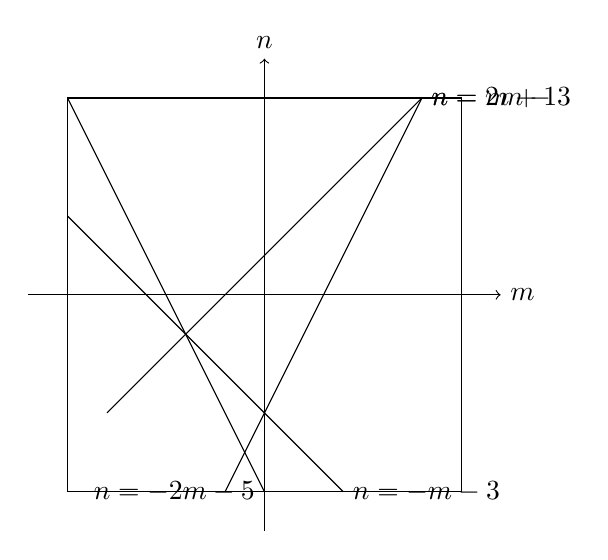
\begin{tikzpicture}[scale=0.5]
\draw[->] (-6,0) -- (6,0) node[right]{$m$};
\draw[->] (0,-6) -- (0,6) node[above]{$n$};
\draw (-5,-5) rectangle (5,5);
\draw[domain=-1:4] plot (\x, {2*\x - 3}) node[right]{$n=2m-3$};
\draw[domain=-5:0] plot (\x, {-2*\x - 5}) node[left]{$n=-2m-5$};
\draw[domain=-5:2] plot (\x, {-\x - 3}) node[right]{$n=-m-3$};
\draw[domain=-4:4] plot (\x, {\x + 1}) node[right]{$n=m+1$};
\end{tikzpicture}
\end{center}

よって $(m, n)$ の組数は
$10 + 8 + 6 + 6 - 4 = 26$ コ

\end{document}
